\documentclass{article}
% Chinese
% \documentclass[UTF8, nofonts, mathptmx, 12pt, onecolumn]{article}
% \usepackage{xeCJK}
% \setCJKmainfont{SimSun}
\usepackage{amsmath}
\usepackage{amsfonts}
\usepackage{amssymb}
\usepackage{wasysym}
\usepackage{ctex}
\usepackage{graphicx}
\usepackage{float}
\usepackage{geometry}
\geometry{a4paper,scale=0.8}
\usepackage{caption}
\usepackage{subcaption}
% \newcommand{\oiint}{\mathop{{\int\!\!\!\!\!\int}\mkern-21mu \bigcirc} {}}
\newcommand*{\dif}{\mathop{}\!\mathrm{d}}
\newcommand*{\md}{\mathop{}\!\mathrm{d}}
\newcommand*{\me}{\mathrm{e}}

\usepackage{parskip}
\setlength{\parindent}{0cm}

\usepackage{bm}
\let\Oldmathbf\mathbf
\renewcommand{\mathbf}[1]{\boldsymbol{\Oldmathbf{#1}}}
\let\eqnarray\align

\author{Xiping Hu}
\usepackage{authblk}
\author{Xiping Hu}
\affil{https://hxp.plus/}
\title{Solution for Test 1}

\begin{document}
\maketitle

\section{Problem 1}

\begin{equation*}
  \begin{aligned}
    \Psi \left( z,t \right) = A \exp \left[ - \left( a^2 z^2 + b^2 t^2 + 2 a b z t \right) \right] = A \exp \left[ - \left( a z + b t \right)^2 \right]
  \end{aligned}
\end{equation*}

波函数

\begin{equation*}
  \begin{aligned}
    \dfrac{\partial^2 \Psi }{\partial x^2 } = \dfrac{1}{v^2} \dfrac{\partial^2 \Psi}{\partial t^2} 
  \end{aligned}
\end{equation*}

求导

\begin{equation*}
  \begin{aligned}
    \dfrac{\partial \Psi}{\partial z} &= A \exp \left[ - \left( a z + b t \right)^2 \right] \cdot \left( - 2 \left( a z + b t \right) \right) \cdot 2 a = - 4 A \exp \left[ - \left( a z + b t \right)^2 \right] \cdot \left(a^2 z + a b t \right) \\
    \dfrac{\partial^2 \Psi}{\partial z^2} &= - 4 A \left\{ \exp \left[ - \left( a z + b t \right)^2 \right] \cdot a^2 - 4 \left( a^2 z + a b t \right)^2 \exp \left[ - \left( a z + b t \right)  \right]\right\} \\
    \dfrac{\partial \Psi}{\partial t} &= A \exp \left[ - \left( a z + b t \right)^2 \right] \cdot \left( - 2 \left( a z + b t \right) \right) \cdot 2 b = - 4 A \exp \left[ - \left( a z + b t \right)^2 \right] \cdot \left(a b z + b^2 t \right) \\
    \dfrac{\partial^2 \Psi}{\partial t^2} &= - 4 A \left\{ \exp \left[ - \left( a z + b t \right)^2 \right] \cdot b^2 - 4 \left( a b z + b^2 t \right)^2 \exp \left[ - \left( a z + b t \right)  \right]\right\} 
  \end{aligned}
\end{equation*}

因此

\begin{equation*}
  \left\{
  \begin{aligned}
    \dfrac{\partial^2 \Psi }{\partial x^2 } &= \dfrac{1}{v^2} \dfrac{\partial^2 \Psi}{\partial t^2} \\
    v &= \dfrac{b}{a}
  \end{aligned}
  \right.
\end{equation*}

波沿z轴正方向传播

\section{Problem 2}

\begin{equation*}
  \begin{aligned}
    \vec{E} = \left( - 6 \hat{\imath} + 3 \sqrt{5} \hat{\jmath}  \right) \left( 10^4 V/m \right) \exp \left\{ i \left[ \dfrac{1}{3} \left( \sqrt{5} x + 2 y \right) \pi \times 10^7 - 9.42 \times 10^{15} t  \right] \right\}
  \end{aligned}
\end{equation*}

显然波是在xy平面传播的,将上面的方程化成如下形式

\begin{equation*}
  \begin{aligned}
    \vec{E} \left( \vec{r}, t \right) = \vec{A} \exp \left[ i \left( \vec{k} \cdot \vec{r} - \omega t \right) \right]
  \end{aligned}
\end{equation*}

\begin{equation*}
  \left\{
  \begin{aligned}
    \vec{A} &= \left( -6, 3 \sqrt{5}, 0 \right) \left( 10^4 V/m \right) \\
    \vec{k} &= \dfrac{\pi}{3} \times 10^7 \times \left( \sqrt{5}, 2, 0 \right) \\
    \omega &= 9.42 \times 10^{15} 
  \end{aligned}
  \right.
\end{equation*}

上述各量的大小为

\begin{equation*}
  \left\{
  \begin{aligned}
    A &=  9 \times 10^4 \  \mathrm{V / m} \\
    k &= \pi \times 10^7 \ \mathrm{m^{-1}}\\
    \omega &= 9.42 \times 10^{15} \  \mathrm{s^{-1}}
  \end{aligned}
  \right.
\end{equation*}

由此求得

\begin{equation*}
  \left\{
  \begin{aligned}
    \lambda &= \dfrac{2 \pi}{k} = 2 \times 10^{-7} \  \mathrm{m} \\
    \kappa &= \dfrac{1}{\lambda} = 5 \times 10^6 \  \mathrm{m^{-1}} \\
    f &= \dfrac{\omega}{2 \pi} = 1.50 \times 10^{15} \  \mathrm{s^{-1}} \\
    \dfrac{\vec{A}}{|A|} &= \left( - \dfrac{2}{3}, \dfrac{\sqrt{5}}{3}, 0   \right) \\
    \dfrac{\vec{k}}{|k|} &= \left( \dfrac{\sqrt{5}}{3}, \dfrac{2}{3},0   \right) 
  \end{aligned}
  \right.
\end{equation*}

\section{Problem 3}

\begin{equation*}
  \begin{aligned}
    \vec{E} = E_0 \hat{\jmath} \cos \left( \dfrac{\pi z}{z_0}  \right) \cos \left( k x - \omega t \right)
  \end{aligned}
\end{equation*}

从电场的表示形式来看,应该是沿着x方向传播的驻波,驻波的振幅随著z的变化而变化。积化和差得到

\begin{equation*}
  \begin{aligned}
    \vec{E} = \dfrac{E_0}{2}  \hat{\jmath} \left[ \cos \left( \dfrac{\pi z}{z_0} + k x - \omega t \right) + \cos \left( \dfrac{\pi z}{z_0} - k x + \omega t  \right) \right]
  \end{aligned}
\end{equation*}

说明这个光波是由两个沿x方向,传播方向相反的光波叠加形成的。

已知$k$,相速度为

\begin{equation*}
  \begin{aligned}
    v_p = \dfrac{\omega}{k} 
  \end{aligned}
\end{equation*}

\section{Problem 4}

\begin{equation*}
  \begin{aligned}
    m_e \ddot{x} + m_e \gamma \dot{x} + m_e \omega_0^2 x = q_e E \left( t \right)
  \end{aligned}
\end{equation*}

等式左边第一项是电子受到的总共的力,第二项是受到的阻力,第三项是线性的回复力。等式右边是电场给电子的力。将

\begin{equation*}
  \begin{aligned}
    E &= E_0 \exp \left( i \omega t \right) \\
    x &= x_0 \exp \left[ i \left( \omega t - \alpha \right) \right]
  \end{aligned}
\end{equation*}

代入

\begin{equation*}
  \begin{aligned}
    - \omega^2 x + i \omega \gamma x + \omega_0^2 x = \dfrac{q_e E_0}{m_e} \exp \left( i \omega t \right) 
  \end{aligned}
\end{equation*}

\begin{equation*}
  \begin{aligned}
    \left[ \left( \omega_0^2 - \omega^2 \right)  + i \omega \gamma \right] x_0 \exp \left[ i \left( \omega t - \alpha \right) \right] = \dfrac{q_e E_0}{m_e} \exp \left( i \omega t \right) 
  \end{aligned}
\end{equation*}

\begin{equation*}
  \begin{aligned}
    \left[ \left( \omega_0^2 - \omega^2 \right)^2  + \omega^2 \gamma^2 \right] x_0 \exp \left[ i \left( \omega t - \alpha \right) \right] = \dfrac{q_e E_0}{m_e} \exp \left( i \omega t \right) \left[ \left( \omega_0^2 - \omega^2 \right) - i \omega \gamma \right]
  \end{aligned}
\end{equation*}

\begin{equation*}
  \begin{aligned}
    x_0 = \dfrac{q_e E_0}{m_e} \dfrac{1}{\left[ \left( \omega_0^2 - \omega^2 \right)^2 + \gamma^2 \omega^2 \right]} \exp \left( i \alpha \right) \left[ \left( \omega_0^2 - \omega^2 \right) - i \omega \gamma \right]
  \end{aligned}
\end{equation*}

\section{Problem 5}

\begin{figure}[H]
  \centering
  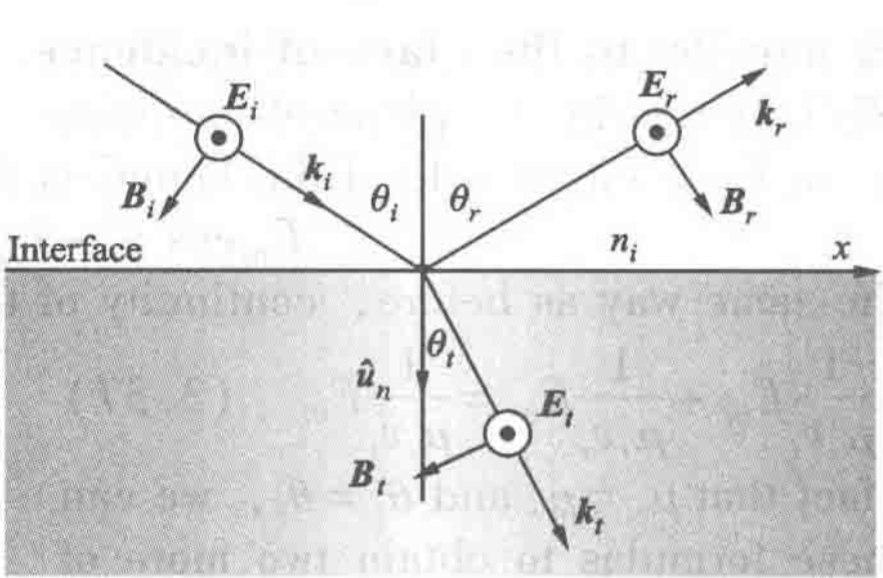
\includegraphics[width=0.5\linewidth]{figures/Fresnel-perpendicular}
  \label{fig:}
\end{figure}

\begin{equation*}
 \left\{
  \begin{aligned}
    & E_i + E_r = E_t \\
    & B_i \cos \theta_i = B_r \cos \theta_r + B_t \cos \theta_t
  \end{aligned}
  \right.
\end{equation*}

\begin{equation*}
  \left\{
  \begin{aligned}
    & E = v B \\
    & v = \dfrac{c}{n}
  \end{aligned}
  \right.
\end{equation*}

\begin{equation*}
 \left\{
  \begin{aligned}
    & E_i + E_r = E_t \\
    & \dfrac{E_i}{v_i}  \cos \theta_i = \dfrac{E_r}{v_r}  \cos \theta_r + \dfrac{E_t}{v_t}  \cos \theta_t
  \end{aligned}
  \right.
\end{equation*}

\begin{equation*}
 \left\{
  \begin{aligned}
    & E_i + E_r = E_t \\
    & n_i E_i \cos \theta_i = n_r E_r \cos \theta_r + n_t E_t \cos \theta_t
  \end{aligned}
  \right.
\end{equation*}

定义

\begin{equation*}
  \begin{aligned}
    r = \dfrac{E_r}{E_i} \\
    t = \dfrac{E_t}{E_i} 
  \end{aligned}
\end{equation*}

则有

\begin{equation*}
 \left\{
  \begin{aligned}
    & 1 + r = t \\
    & n_i \cos \theta_i = n_r r \cos \theta_r + n_t t \cos \theta_t
  \end{aligned}
  \right.
\end{equation*}

解得菲涅耳公式

\begin{equation*}
  \left\{
  \begin{aligned}
    r_{\perp} = \dfrac{n_i \cos \theta_i - n_t \cos \theta_t}{n_i \cos \theta_i + n_t \cos \theta_t} \\
    t_{\perp} = \dfrac{2 n_i \cos \theta_i}{n_i \cos \theta_i + n_t \cos \theta_t} 
  \end{aligned}
  \right.
\end{equation*}


又因为 $n_i \sin \theta_i = n_t \sin \theta_t$

\begin{equation*}
  \left\{
  \begin{aligned}
    r_{\perp} &= \dfrac{n_i \cos \theta_i - n_t \cos \theta_t}{n_i \cos \theta_i + n_t \cos \theta_t} = \dfrac{\cos \theta_i - \dfrac{n_t}{n_i}  \cos \theta_t}{\cos \theta_i + \dfrac{n_t}{n_i}  \cos \theta_t} = \dfrac{\cos \theta_i - \dfrac{\sin \theta_i}{\sin \theta_t}  \cos \theta_t}{\cos \theta_i + \dfrac{\sin \theta_i}{\sin \theta_t}  \cos \theta_t} = \dfrac{\sin \theta_t \cos \theta_i - \sin \theta_i \cos \theta_t}{\sin \theta_t \cos \theta_i + \sin \theta_i \cos \theta_t} \\
    t_{\perp} &= \dfrac{2 n_i \cos \theta_i}{n_i \cos \theta_i + n_t \cos \theta_t} = \dfrac{2 \cos \theta_i}{\cos \theta_i + \dfrac{n_i}{n_t}  \cos \theta_t} = \dfrac{2 \cos \theta_i}{\cos \theta_i + \dfrac{\sin \theta_i}{\sin \theta_t}  \cos \theta_t} = \dfrac{2 \sin \theta_t \cos \theta_i}{\sin \theta_t \cos \theta_i + \sin \theta_i \cos \theta_t}
  \end{aligned}
  \right.
\end{equation*}

即

\begin{equation*}
  \left\{
  \begin{aligned}
    r_{\perp} &= \dfrac{\sin \left( \theta_t - \theta_i \right)}{\sin \left( \theta_i + \theta_t \right)} \\
    t_{\perp} &= \dfrac{2 \sin \theta_t \cos \theta_i}{\sin \left( \theta_i + \theta_t \right)} 
  \end{aligned}
  \right.
\end{equation*}

\begin{equation*}
  \begin{aligned}
    t_{\perp} - r_{\perp} = \dfrac{2 \sin \theta_t \cos \theta_i}{\sin \left( \theta_i + \theta_t \right)} - \dfrac{\sin \left( \theta_t - \theta_i \right)}{\sin \left( \theta_i + \theta_t \right)} = \dfrac{2 \sin \theta_t \cos \theta_i - \sin \theta_t \cos \theta_i + \sin \theta_i \cos \theta_t}{\sin \theta_i \cos \theta_t + \sin \theta_t \cos \theta_i} = 1
  \end{aligned}
\end{equation*}

\section{Problem 6}

\begin{figure}[H]
  \centering
  \begin{subfigure}{.5\textwidth}
    \centering
    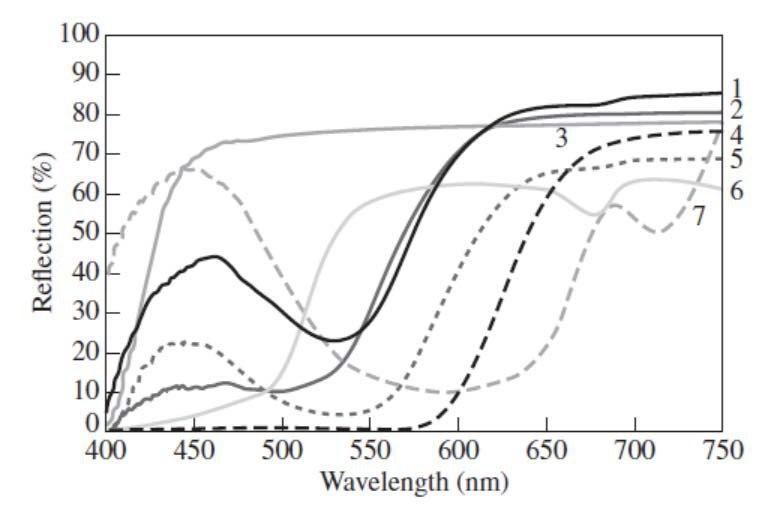
\includegraphics[width=\linewidth]{figures/Spectrum1}
    \label{fig:}
  \end{subfigure}%
  \begin{subfigure}{.5\textwidth}
    \centering
    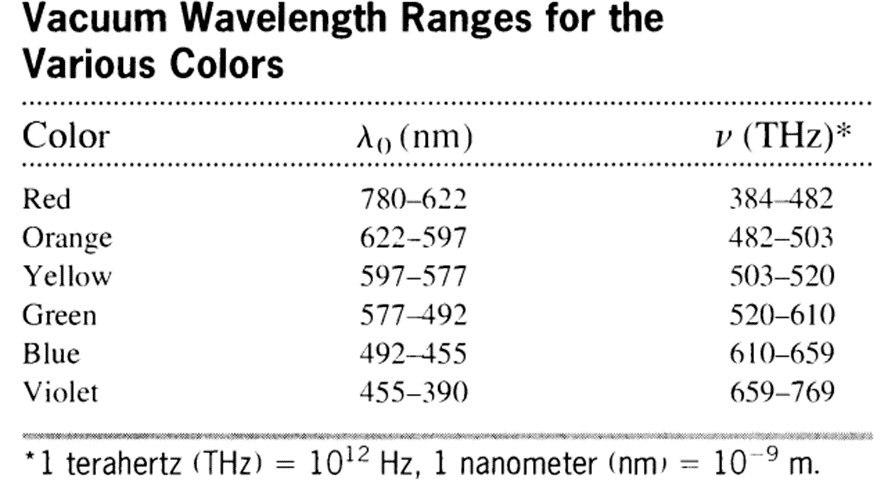
\includegraphics[width=\linewidth]{figures/Spectrum2}
    \label{fig:}
  \end{subfigure}
  \label{fig:}
\end{figure}

白色的是3,反射光里面各种波长都有。

黄色的是6,粉色由红色和蓝色混合而成,应该是1,蓝色是7,橘红色是5,红色是4。


\end{document}